\documentclass[openany,oneside,12pt]{book}
\usepackage{hyperref}
\usepackage{amsmath}
\usepackage[utf8]{inputenc}
\usepackage{tcolorbox}
\usepackage{listings}
\usepackage{listings-golang} % import this package after listings
\usepackage{color}
\usepackage{amssymb}
\usepackage{tikz}
\usetikzlibrary{positioning}
\lstset{
	language=Golang,
	aboveskip=3mm,
	belowskip=3mm,
	showstringspaces=false,
	columns=flexible,
	basicstyle={\small\ttfamily},
	numbers=none,
	numberstyle=\tiny\color{gray},
	keywordstyle=\color{blue},
	commentstyle=\color{red},
	stringstyle=\color{red},
	breaklines=true,
	breakatwhitespace=true,
	tabsize=3}
\title{MFree: An Explicit Meshfree Code for Non-Linear Solid Mechanics \\ release 0.1}
\date{2018 \\ October}
\author{Stephen Smith \\ Queen's University Belfast}



\newcommand*{\rttensor}[1]{\overline{\overline{#1}}}
\newcommand*{\rttensortwo}[1]{\ubar{\ubar{#1}}}

\raggedbottom
\begin{document}
\frontmatter
\vbox{
	\centering
		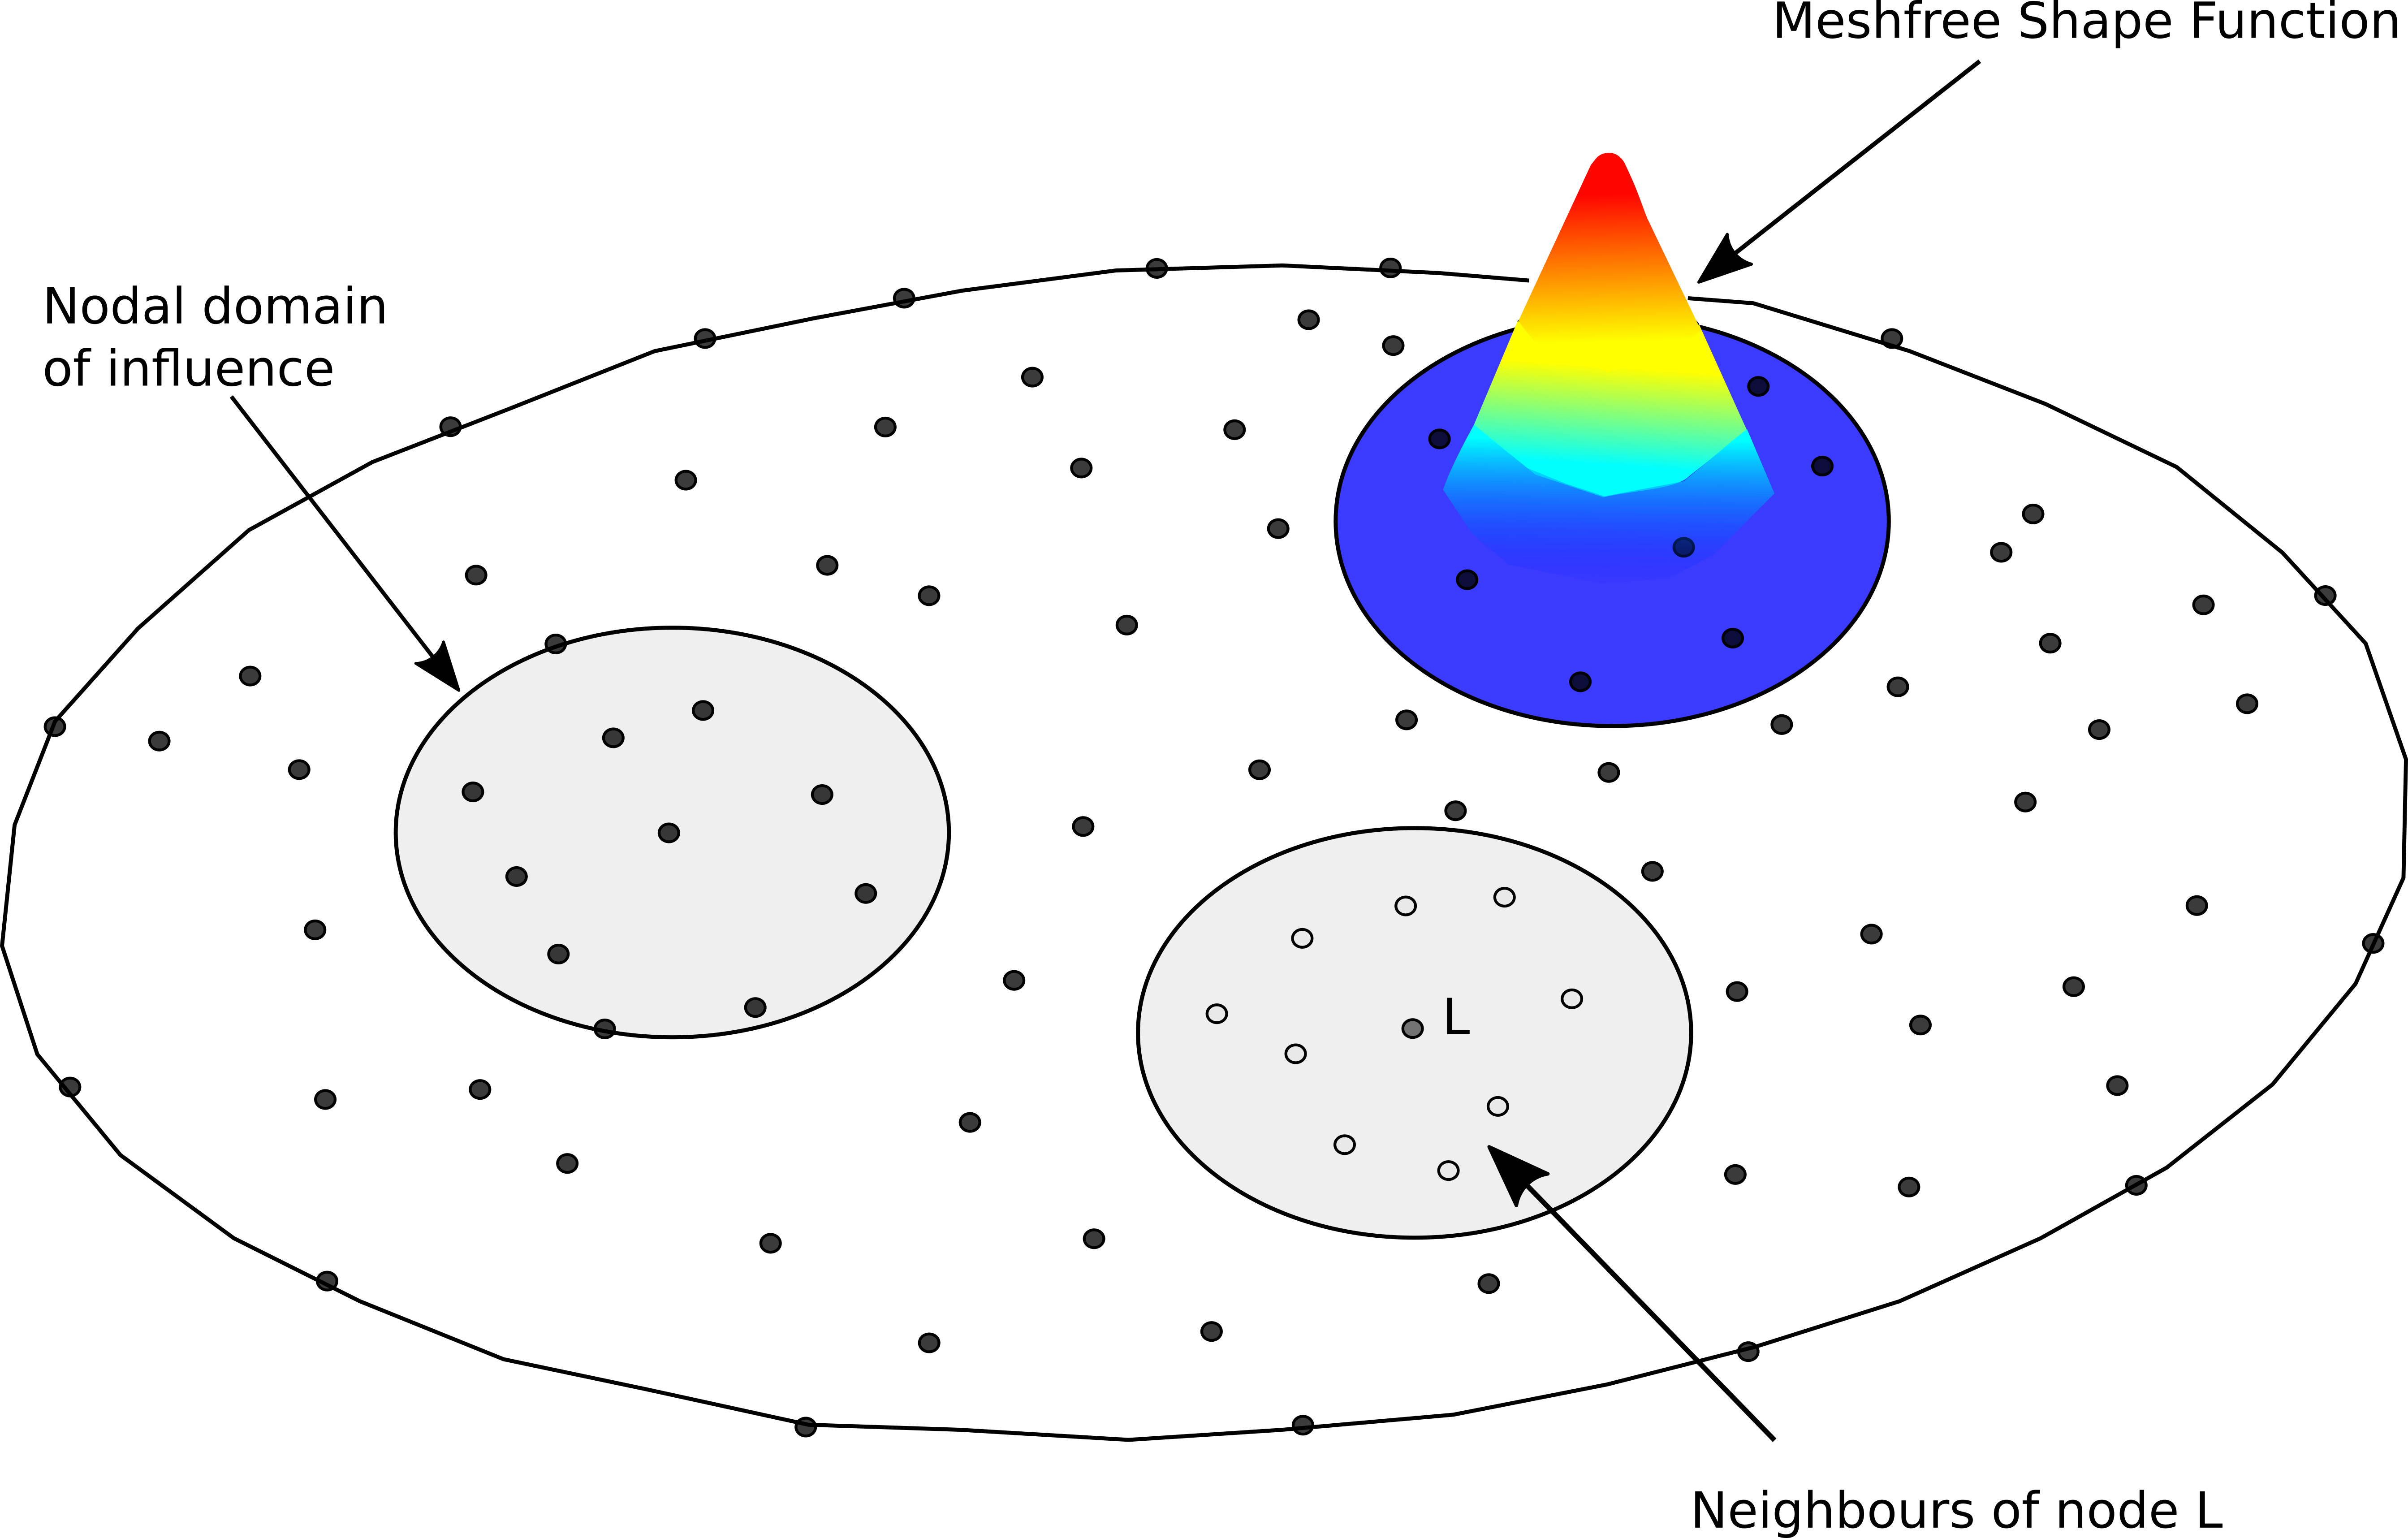
\includegraphics[width=0.9\textwidth,keepaspectratio]{MeshfreeDisc}
	\maketitle %this typesets the contents of \title, \author and \date
}
\tableofcontents
\mainmatter
\chapter{Introduction}
\section{MFree}
The Mfree libary is a framework developed in Cfor mesh-free modelling in a research environment. It was developing during my PhD for application to stretch blow moulding a manufacturing technique used to produce polymer bottles. The main features of the code are the ability to simulate non-linear solid mechanics problems using an explicit solver. The use of the MFree library is intended to simplify the use of mesh-free methods within a research context, and further provide a learning resource for meshfree methods. 

To facilitate this goal, this manuscript has been created in order to describe the main features of this code.
\section{Overview}





\chapter{Theory}		
In order to understand how to use the library it is necessary to have an appreciation of the theory behind the application of meshfree methods to non-linear solid mechanics. This chapter explains the fundamental ideas of meshfree methods, and discretization of a continous problem in a discrete, and numerically solvable one. 
\section{Meshfree methods}
Meshfree methods were developed in the middle of the 1990's to overcome difficulties associated with the finite element method. The fundamental problem in meshfree or finite elements is to provide a set of approximation function (subject to a set of constraints) that can be used as an approximation space for the trial and test functions in the weak form of a partial different equation.  To illustrate this problem, consider the balance of linear momentum, cast in a Lagrangian(reference) form Eq. (\ref{Balance of linear momentum}). The intention in this manuscript is to use capital symbols to describe material coordinates, however often irregularities will exist between this intention and the result. 
\begin{equation}\label{Balance of linear momentum}
\text{GRAD} ~ P_{iJ} = \rho_0 \ddot{u_i}
\end{equation}
where $P$ is the first Piola-Kirchoff stress, $\rho_0$ the material density in the reference frame (typically $t=0$) and $\ddot{u}$ the acceleration. To complete the balance of linear moemntum boundary conditions must be specified. A boundary is called a displacemnt boundary, denoted $\Gamma_u$, if a displacement $u$ is prescribed on that boundary, likewise a similar defintion is present for the traction boundary, denoted $\Gamma_t$ The boundary conditions for Eq. (2.1) are typically given as:
\begin{equation}
u_i=\bar{u_i} ~~on ~~\Gamma_u
\end{equation}
\begin{equation}
P_{ij}N_j = \bar{T_i} ~~on ~~\Gamma_t
\end{equation}
Equation 2, subject to the boundary conditions (2.2,2.3) is often termed the strong form 

	
\begin{tcolorbox}
\textbf{Strong form of the momentum balance}
\begin{align*}
\text{GRAD} ~ P_{iJ} &= \rho_0 \ddot{u_i} &\text{Momentum Balance} \\
u_i&=\bar{u_i} ~~on ~~\Gamma_u &\text{Displacement condition} \\
P_{ij}N_j &= \bar{T_i} ~~on ~~\Gamma_t &\text{Traction condition}
\end{align*}
\end{tcolorbox}

\subsection*{Strong form to weak form }
To construct the weak form a test function $\delta u$ is introduced, which is assumed to be smooth enough up to the required order of the problem, and vanishes on the displacement boundary. The strong form, denoted $\mathcal{S}(u)$ of Box 1 is now cast into an alternate, but equivalent problem: 
\vspace{0.5cm}

\noindent\emph{Given a strong form $\mathcal{S}(u)$, find the trial dispalcemnt field $u(X,t)$ such that the following equation is satisfied }
\begin{equation}
\int{\delta u_i \cdot [GRAD ~P_{iJ} - \rho_0 \ddot{u}     ] d\Omega} = 0
\end{equation}
which is obtained from integrating the product of the strong form $S(u)$ and the test functions $\delta u$. Expanding (2.4) using the product rule of integration leads to the following form: 
\begin{equation}
\int{\big(\text{GRAD}~\delta u_i P_{iJ} + \delta u_i \rho_0 \ddot{u}_i \big) d\Omega     } - \int{\bar{T_i} \delta u_i d \Gamma_t} = 0
\end{equation}
This form of the equation can conveniently (for the sake of physical interpretation) be cast into the the principle of virtual work:
\begin{align}
\delta W &= \delta W^{int} - \delta W^{ext} + \delta W^{kin} 
\end{align}
Before summarising the derivation it is necessary to make a note on the definition of the trial and test functions. Firstly as mentioned above the test functions $\delta_u$ should vanish on the displacement boundary, and be continuous up to order required, which in the above form requires the existence of the first derivatives. With reference to this we define the space of functions $\mathcal{U}_0$ that satisfy these conditions:
\begin{equation}
\delta u(X) \in \mathcal{U}_0 ~~ \text{where} ~~ \mathcal{U}_0 = \{ \delta u(X) | \delta u(X) \in C^0(X), \delta u = 0 ~on~ \Gamma_u         \}
\end{equation}
In a similar manner the functions space for the trial functions $u(X,t)$ can be defined, with the condition that the displacemnt boundary conditions are satisfied. 
\begin{equation}
 u(X,t) \in \mathcal{U} ~~ \text{where} ~~ \mathcal{U} = \{u(X,t) | u(X,t) \in C^0(X), u(X,t) = \bar{u} ~on~ \Gamma_u         \}
\end{equation}
Combining these definitions with the principle of virtual work above leads to the complete problem, given by:
\begin{tcolorbox}
	\textbf{Principle of virtual work (Weak form)}
	Find the trial functions $u(X,t)$ such that for any admissible (member of $\mathcal{U}_0$) virtual displacement $\delta u$ the virtual work $\delta W $ is zero.
	\begin{equation*}
	\delta W = \delta W^{int} - \delta W^{ext} + \delta W^{kin} 
	\end{equation*}
	where 
	\begin{align*}
	\delta W^{int} &= \int{\text{GRAD}~\delta u_i P_{iJ}d \Omega} \\
	\delta W^{ext} &=  \int{\bar{T_i} \delta u_i} d \Gamma_t \\
	\delta W^{kin} &= \int{\delta u_i \rho_0 \ddot{u}_i d \Omega}
	\end{align*}
\end{tcolorbox}
\subsection*{Discretization}
The weak form in Box 2 still requires the determination of the continuous function $u(X,t)$ which in most cases will be impossible. A set of discrete equations can be developed by considering an approximation of the displacements, which in its most general form: \emph{Given a set of data points $X \in \mathcal{R}^d$, with nodal values $u_d$}. Any approximation scheme is subject to a minimum of two constraints in order to be applied to the virtual work statement above:
\begin{tcolorbox}
\textbf{	Shape function requirements}
	\begin{enumerate}
		\item The shape functions should be able to reproduce a constant field
		\begin{equation*}
		\implies \sum_I \phi_I = 1
		\end{equation*}
		\item In order to ensure first order convergence the shape functions should be able to reproduce a polynomial
		\begin{equation*}
		\implies \sum_I \phi_I x_{kI} = x_k ~~ for~k=1,2,3
		\end{equation*}
	\end{enumerate}
\end{tcolorbox}
\noindent This leads to the following form

\begin{equation}
u(X,t) = \sum_I^N \phi_I(X) u_{Ii}(t)
\end{equation}
and the derivative by:
\begin{equation}
u(X,t),_J = \sum_I^N \phi_I(X),_J u_{Ii}(t) ~~where~j = 1,..,n_d
\end{equation}
The construction of the shape functions $\phi_I$ is dependent on the method used. If the data points X are arranged into convex polygons, then the shape functions coincide with those used in the finite element method. However, this predefined computational mesh can create issues in large deformation, which lead to the develop of meshfree approximation methods. In this case an arbitrary, but local support is assigned to each node Fig. 1. The simplest shape function that can be constructed for this domain is the shepard function, defined by a ratio of the weight functions
\begin{equation}
\phi_i = \frac{\omega_a (x; x-x_i)}{\sum_j^n \omega_a(x;x-x_j)} 
\end{equation}
which clearly satisfies the first condition (constant reproduction) as
\begin{equation}
\sum_i \phi_i = \frac{\sum_i^n\omega_a (x; x-x_i)}{\sum_j^n \omega_a(x;x-x_j)} = 1
\end{equation}
However, in order to satisfy the linear reproducing conditions an additional enrichment term is required. This is typically ahcieved by introducing a monomial basis terms into the approximation, yieding a general form of meshfree shape functions
\begin{equation}
u^h(x) = \sum_i^n C_i(x) \Gamma_i(x)
\end{equation}
where $\omega$ is a weight function, and $C_I$ corrective terms, which meet the reproducing conditions. 
However, in order to satisfy the linear reproducing conditions an additional enrichment term is required. Consider the general form of the meshfree aporixmation given by 
However, in order to satisfy the linear reproducing conditions an additional enrichment term is required. Consider the general form of the meshfree aporixmation given by 
However, in order to satisfy the linear reproducing conditions an additional enrichment term is required. Consider the general form of the meshfree aporixmation given by 
\subsubsection*{Probabilistic Approach}
The approach above for developing meshfree shape functions leads to one drawback, the shape functions no longer interpolate data, which presents problems in implementing boundary conditions. In order to fix this issue a probablistic approach to mesh-free shape functions was developed by Ortiz \cite{}, known as the MAXENT scheme. In this approach we consider the shape function approximation form $u^h(x) = \phi_I u_I$ and associate the shape function with a probability, we interpret the shape functions $\phi_I$ as \emph{the probability $p_I$ to which point $I$ influences $x$}, then the shape function approximation gives the expected value $\sum \phi_I u_I = \mathcal{E}(u)$. In order to find the probablity distrubitoon ( or shape functions) the principle of maximum entropy is used, which states for a given probability distribution $\phi_i$ with $\sum_i \phi_i = 1$ then the least biased distribution is the one that maximises information entropy is given by 
\begin{tcolorbox}
\textbf{Principle of maximum entropy (MAXENT):}
\begin{equation*}
\max_{\phi_I} ~~H(\phi_i) = - \sum_i \phi_i log(\phi_i)
\end{equation*}
\end{tcolorbox}
\noindent subject to the reproducing constraints (in 2D):
\begin{equation*}
\sum_I \phi_I = 1, ~~~~\sum_I \phi_I x_{Ik} = x_k, 
\end{equation*}
The constaints are added to the MAXENT principle uisng Lagrange multipliers, which produces the following Lagrangian:
\begin{equation}
\delta ~\bigg[\sum_I -\phi_I log \phi_I + \lambda_0 ( 1- \sum_I \phi_i)+ \lambda_k ( x_k- \sum \phi_I x_{Ik})\bigg]  = \mathbf{0}
\end{equation}
simplifying 2.14 and using the relation $ \lambda_0 = log(Z) - 1$ yields the following:
\begin{equation}
\phi_I = \frac{e^{-( \lambda_k x_{Ik})    }}{Z}, ~~~ Z(\lambda_k) = \sum_I e^{-( \lambda_k x_{Ik})    }
\end{equation}
subject to the $k$ constraints:
\begin{equation}
f_k(\lambda_k) = \frac{\sum e^{-( \lambda_k x_{Ik})    }}{Z} - x_k ~~ \text{for} ~k = (1,...,nd)
\end{equation}
For numerical reasons (give some?) introducing the shifted coordinates $\tilde{x_{Ik}} = x_{Ik} - x_k$ is advantageus as it casts the maximisation into the dual problem of minimization. In the shifted coordinates the $k$ constraints are:
\begin{equation}
\sum_I \phi_I \tilde{x}_{kI} = 0
\end{equation} 
and $\phi$ and $\tilde{Z}$
\begin{equation}
\phi_I = \frac{e^{-(\lambda_k \tilde{x}_{Ik})}}{\tilde{Z}}, ~~~~ \tilde{Z} = \sum_I e^{-(\lambda_k \tilde{x}_{Ik})}
\end{equation}
Substitution of Eqs 2.18 into the MAXENT principle yields:
\begin{equation}
H_{max} = log(\tilde{Z})
\end{equation}
subject to the constraints
\begin{equation}
\frac{\partial log(\tilde{Z)}}{\partial \lambda_k} = 0
\end{equation}
Hence, the solution to this problem is as follows: \emph{Find the set of Lagrange multipliers ($\lambda_k$) that minimise the convex potential function $F(\lambda_k) = H_{max}$}. This problem is solved iteratively using schemes such as \textit{steepest-descent method} or \textit{Newton-Raphson} methods. 
\begin{tcolorbox}
\textbf{MAXENT Construction in 2D:}
Goal: Minimise the convex potential function $F(\lambda_1,\lambda_2) = log(\sum_I e^{-\lambda_1 \tilde{x}_i - \lambda_2 \tilde{y}_i})$. Method: Assume that the solution $\lambda^k$ at the $kth$ iteration is given, then the minimisation problem can be expanded using a Taylor series
\begin{equation*}
F(\lambda^k+\Delta \lambda^k) = \mathcal{R}(\lambda^k) + \nabla \nabla F(x) \Delta \lambda^k = 0
\end{equation*}
where $\mathcal{R}$ is the residual at the $kth$ iteration:
\begin{equation*}
\mathcal{R} = \nabla F(\lambda_1^k,\lambda_2^k) > 0 
\end{equation*}
The increment $\Delta \lambda^K$ at the $kth$ iteration is given by:
\begin{equation*}
\Delta \lambda^k = -\mathcal{H}^{-1} \nabla F
\end{equation*}
Where $\mathcal{H}$ is the Hessian matrix $(\mathcal{H}:=\nabla^2 F)$. After convergence is reached, subject to a tolerance, the shape functions are given by:
\begin{equation}
\phi_i = \frac{e^{\lambda_1 x_i - \lambda_2 y_i}}{\sum_{j=1}^ne^{\lambda_1 x_j - \lambda_2 y_j} } 
\end{equation}
Eqs (2-3) describe a Newton-Raphson scheme.
\end{tcolorbox}

\subsection*{Discrete Equations}
To form the discrete equations used in the meshfree simulation we now subsitute the shape function approximation of the displacement eq. (5) into the virtual work expression, Box 2. As this is a Galerkin method the same basis functions are used for the trial and test functions, such that:
\begin{equation}
u_i^h = \sum_I \phi_I u_{Ii} , ~~~ \delta u_i = \sum_I \phi_I \delta u_{Ii}
\end{equation}
Considering the virtual work expression evaluated at a point $X_L$, Fig 3. The $n$ nodes that influence of the point x is given by the set:
\begin{equation}
\mathcal{I}_L = \{x_I : w(x-X_I) > 0 \}
\end{equation}

\begin{figure}
	\centering
	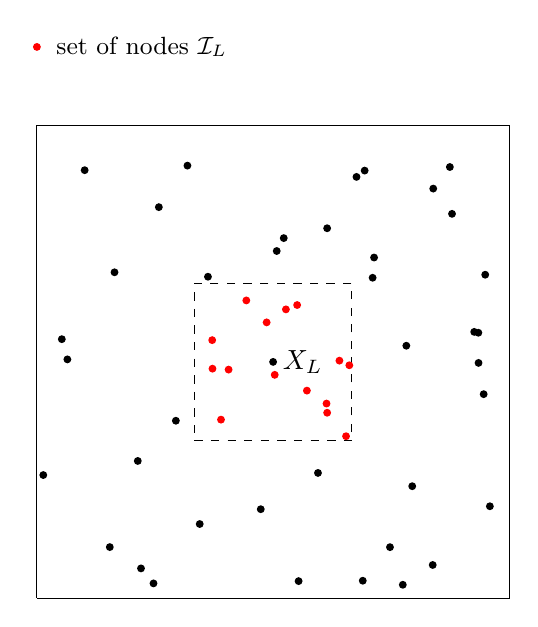
\begin{tikzpicture}
	\draw (-3,-3) -- (3,-3) -- (3,3) -- (-3,3) -- (-3,-3);
	\begin{scope}
	\clip (-3,-3) rectangle +(6,6);
	\pgfmathsetseed{24122015}
	\foreach \p in {1,...,100}
	{ \fill (5*rand,5*rand) circle (0.05);
	}
	\end{scope}
	\draw[dashed,fill=white] (-1,-1) -- (1,-1) -- (1,1) -- (-1,1) -- (-1,-1);
		\pgfmathsetseed{241210101}
	\foreach \p in {1,...,15}
	{ \fill[red] (1*rand,1*rand) circle (0.05);
		}
	\fill[black] (0,0) circle(0.05) node[right] {$X_L$};
	\fill[red] (-3,4) circle (0.05) node (m1) [label={[black]right:\small{set of nodes $\mathcal{I}_L$}}] {};

	\end{tikzpicture}	
	\caption{Virtual work at a point $X_L$}
\end{figure}
\noindent And therefore the displacement given by:
\begin{equation}
u_i(x_L) = \sum_I \phi_I(X_L) u_{Ii} ~~~ \text{for}~I \in \mathcal{I}_L 
\end{equation}
or given by the k vector equations
\begin{equation}
{u_K(X_L)} = \mathbf{\Phi}^T\mathbf{u}_k =  <\phi_I,...,\phi_N>\cdot <u_{1k},...,u_{Nk}>^T
\end{equation}
where $\text{len}(\mathbf{u}) =  card(\mathcal{I}_L)$. The derivatives of u can be developed in a similar manner
\begin{equation}
\frac{\partial u_k(X_L) }{\partial X_J} = \Phi_{,J}^T u_k = \mathbf{g}^T_J \mathbf{u}_k
\end{equation}
The first term of the internal virtual work ($GRAD ~\delta u$) can hence be evaluated as 
\begin{equation}
(GRAD~ \delta u)_{kJ} = \frac{\partial \delta u_k}{\partial  X_J} = \begin{array}{c} \begin{bmatrix}
\mathbf{g}_1^T \delta \mathbf{u}_1       & \mathbf{g}_2^T \delta \mathbf{u}_1 & \mathbf{g}_3^T \delta \mathbf{u}_1   \\
\mathbf{g}_1^T \delta \mathbf{u}_2       & \mathbf{g}_2^T \delta \mathbf{u}_2 & \mathbf{g}_3^T \delta \mathbf{u}_2     \\
\mathbf{g}_1^T \delta \mathbf{u}_3       & \mathbf{g}_2^T \delta \mathbf{u}_3 & \mathbf{g}_3^T \delta \mathbf{u}_3
\end{bmatrix}\\
\mathbf{G}
\end{array}
\end{equation}
For computational reasons (give some) it is necessary to transform 2.27 into a matrix-vector equations, by means of Voigt notation, which reduces a second order tensor (such as the deformation gradient) into a vector, and a fourth order tensor (such as the material stiffness tensor) into a matrix. 
\begin{tcolorbox}
\textbf{Voigt Notation:}
\begin{align*}
\{F\} &= Voigt\bigg(\begin{bmatrix}
F_{11} &F_{12} &F_{13} \\
F_{21} &F_{22} &F_{23} \\
F_{31} &F_{32} &F_{33} 
\end{bmatrix}\bigg) \\
&= <F_{11},F_{22},F_{33},F_{23},F_{13},F_{12},F_{21},F_{31},F_{32}>^T
\end{align*}
or for symmetric tensors 
\begin{align*}
\{S\} &= Voigt\bigg(\begin{bmatrix}
S_{11} &S_{12} &S_{13} \\
S_{21} &S_{22} &S_{23} \\
S_{31} &S_{32} &S_{33} 
\end{bmatrix}\bigg) \\
&= <S_{11},S_{22},S_{33},S_{23},S_{13},S_{12}>^T
\end{align*}
\end{tcolorbox}
Using Voigt notation, and after some manipulation with row padding, the following form of the virtual deformation gradient is given by:
\begin{equation}
\{GRAD ~\delta u\}_K = \begin{array}{c}\begin{bmatrix}
g_{11}       & 0 & 0 & \dots & g_{N1} & 0 & 0 \\
0       & g_{21} & 0 & \dots & 0 & g_{N2} & 0 \\
0       & g_{21} & 0 & \dots & 0 & g_{N2} & 0 \\
0       & g_{21} & 0 & \dots & 0 & g_{N2} & 0 \\
0       & g_{21} & 0 & \dots & 0 & g_{N2} & 0 \\
0       & g_{21} & 0 & \dots & 0 & g_{N2} & 0 \\
0       & g_{21} & 0 & \dots & 0 & g_{N2} & 0 \\
0       & g_{21} & 0 & \dots & 0 & g_{N2} & 0 \\
0       & g_{21} & 0 & \dots & 0 & g_{N2} & 0 
\end{bmatrix}\\
\mathbf{B_I}(X_L)
\end{array}\begin{array}{c}\begin{bmatrix}
\delta u_{11} \\
\delta u _{12} \\
\delta u_{13} \\
\vdots \\
\vdots \\

\delta u_{N1} \\
\delta u _{N2} \\
\delta u_{N3} 
\end{bmatrix}

\end{array}
\end{equation}
where $g_{IJ} = \frac{\partial \phi_I}{\partial X_J}$. The matrix $B$ is known as the strain-displacement matrix, and after applying Voigt notation to the 1PKF stress, P yields the following form of the internal force
\begin{equation}
\delta W^{int} = \int {(B\delta u)^T {P} d \Omega}
\end{equation}
As $\mathbf{\delta u}$ is not a function of the material coordinates it can be taken out of the integral,
\begin{align}
a &=  \\
\implies b &= 0
\end{align}
\section{Constitutive Modelling}
An essential stage in the solution of the virtual work expression, Box 2, is to relate the trial displacement field $u(X,t)$ to the stresses. This is made possible through the use of a constitutive equation. The simplest form of a constitutive law for large strain is the St Venant-Kirchoff law, which is linear in the strain measure (but not the displacements due to the non-linear relationship between the strains and the displacements), represented by the equation:
\begin{equation}
S_{IJ} = \lambda E_{KK}\delta_{KK} \delta_{IJ} + 2\mu E_{IJ}
\end{equation}
Materials such as this one are part of a general class of materials known as hyper-elastic materials, where the constitutive law is given in terms of a strain energy density function $\Psi$. For example, the strain energy density function for the St. Venant Kirchoff material is given by:
\begin{equation}
\psi(E_{IJ}) = \frac{\lambda}{2}\big[E_{IJ} : \delta_{MN} \big]
\end{equation}
In general the strain energy density function for isotropic hyper-elastic models is defined in terms of the invariants of the right Cauchy-Green tensor $C$, given by
\begin{align*}
I_1 &= tr(C) \\
I_2 &= (tr(C))^2 - tr(C^2)\\
I_3 &= det(F)\\
\end{align*}
The routine for defining, or using a hyper-elastic is as follows
\begin{tcolorbox}
\textbf{Hyperelastic Material:}
Given a functional relationship between the strain energy density function, and the invariants $I_1,I_2,I_3$ of the right-Cauchy deformation tensor, the Cauchy stress can be obtained from the following:
\begin{equation}
\sigma = \frac{2}{J}\bigg(\frac{\partial \Psi}{\partial I_1}\bigg)
\end{equation}

\end{tcolorbox}


\section{Integration}
In order to solve the virtual work expression integration is required, in order to achieve this in the finite element method Gauss integration is typically used. However, the application of the Gauss integration to meshfree methods leads to poor performance, due the fact that meshfree shape functions are not polynomials, and also have an arbitrary supports, which does not necessarily align with the integration structure. In response to this different integration schemes have been proposed, such as support integration, stress point nodal integration and corrected gauss integration. In this library stabilised nodal integration is used, which ensures that the first order reproducing conditions of the shape functions are met, Box 3. This condition imposes a restriction on the integration scheme, which can be shown by considering a linear patch test, Fig 2,
\begin{figure}
	\centering
	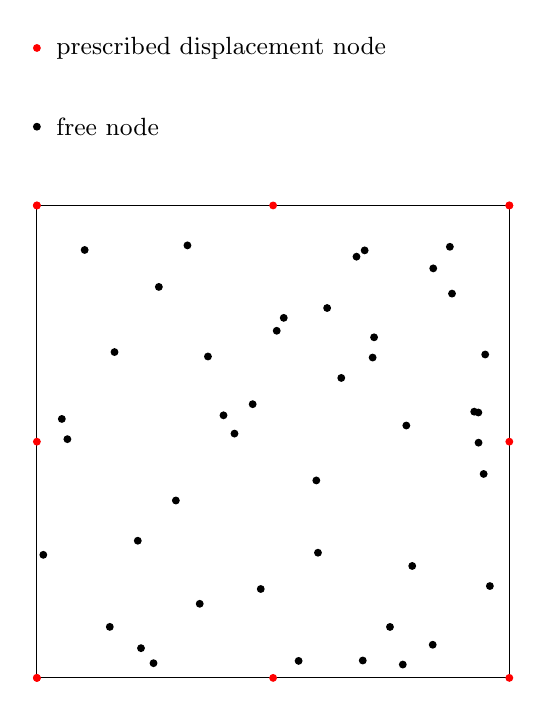
\begin{tikzpicture}
	\draw (-3,-3) -- (3,-3) -- (3,3) -- (-3,3) -- (-3,-3);
	\begin{scope}
	\clip (-3,-3) rectangle +(6,6);
	\pgfmathsetseed{24122015}
	\foreach \p in {1,...,100}
	{ \fill (5*rand,5*rand) circle (0.05);
	}
	\end{scope}
	% nodes on boundary
	\fill[red] (3,-3) circle (0.05);
	\fill[red] (3,0) circle (0.05);
	\fill[red] (3,3) circle (0.05);
	\fill[red] (3,3) circle (0.05);
	\fill[red] (0,-3) circle (0.05);
	\fill[red] (-3,-3) circle (0.05);
	\fill[red] (-3,3) circle (0.05);
	\fill[red] (0,3) circle (0.05);
	\fill[red] (-3,-3) circle (0.05);
	\fill[red] (-3,0) circle (0.05);
	\fill[red] (-3,3) circle (0.05) ;
	
	
	\fill[red] (-3,5) circle (0.05) node (m1) [label={[black]right:\small{prescribed displacement node}}] {};
	\fill[black] (-3,4) circle (0.05) node (m1) [label={[black]right:\small{free node}}] {};
	\end{tikzpicture}	
	\caption{Patch Test }
\end{figure}
where a linear displacement field  is prescribed on the displacement boundary $\Gamma_u$, given by:


\begin{equation}
u_{iI} = a_{i0} + a_{ij}x_{jI} ~~ \text{for I on } \Gamma_u
\end{equation}
In order to satisfy the patch test, the meshfree solution should be given by a linear polynomial $u_i = a_{i0} + a_{ij}x_j$, and hence the strains by:
\begin{align*}
\epsilon_x &= u_{x,x} = a_{x1} \\
\epsilon_y &= u_{x,x} = a_{y2} \\
2\epsilon_{xy} &= u_{x,y} + u_{y,x} = a_{x2} + a_{y1} 
\end{align*}
which are constant throughout the domain, hence the stress $\sigma^c$ is also constant. Considering the small-strain virtual work expression, with no inertial term (equivalent to the except the use of the small strain tensor $\epsilon := sym(\nabla u)$, and Cauchy stress $\sigma$), the virtual work is given by:
\begin{equation}
\int {B_I^T {\sigma} d \Omega }  = \int{\phi_I t_i d \Gamma_t}
\end{equation}
As the boundary is unloaded, $\int \phi_I t_i d\Gamma_t = 0$, leading to the condition:

\begin{tcolorbox}
\textbf{	Divergence-free Condition:}
\begin{align*}
\int {B_I d\Omega } &= 0 ~~ \text{for}~~ 
\end{align*}
\end{tcolorbox}
If the integration in 2.36 is undertaken using Gauss integration the condition, which leads to poor convergence. In order to create an integration scheme that will satisfy this condition it is necessary redefine the strain displacement matrix B. This is achieved by considering smoothing of the strain over a representative volume, which for the case of the small strain tensor $\epsilon$ is given by:
\begin{equation}
\bar{\delta \epsilon} = \frac{1}{A_L} \int { sym(\nabla \delta u) } d\Omega_L
\end{equation}
which through divergence theorem, can be related to the flux across the surface
\begin{equation}
\bar{\delta \epsilon} = \frac{1}{A_L} \int {\frac{1}{2}(\delta u_i \cdot n_j + \delta u_j \cdot n_i) d\Gamma_L}
\end{equation}
where $n_j$ are the components of the surface normals.

\begin{figure}
	\centering
	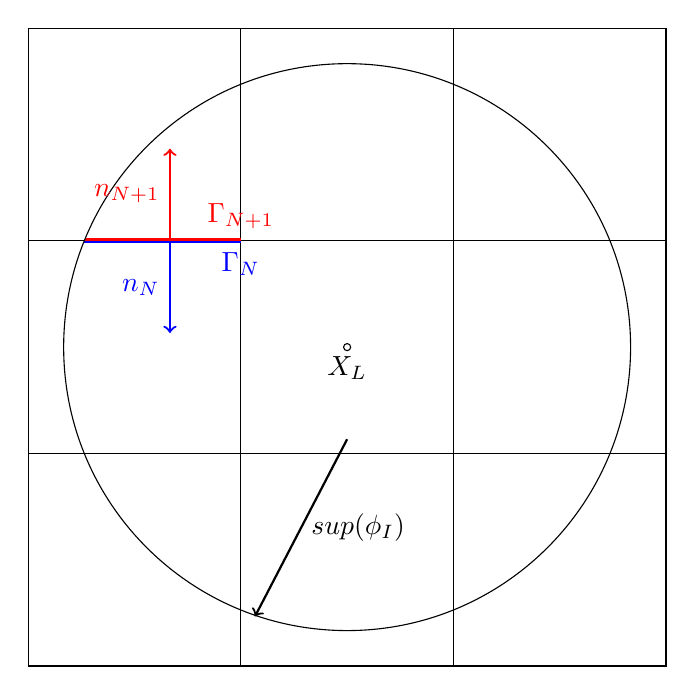
\begin{tikzpicture}[scale=0.9]
	%top row
	\draw (-3,0) rectangle +(3,3);
	\draw (0,0) rectangle +(3,3);	
	\draw (3,0) rectangle +(3,3);
	% middle row
	\draw (-3,-3) rectangle +(3,3);
	\draw (0,-3) rectangle +(3,3);
	\draw (3,-3) rectangle +(3,3);
	% bottom
	\draw (-3,-6) rectangle +(3,3);
	\draw (0,-6) rectangle +(3,3);
	\draw (3,-6) rectangle +(3,3);
	
	
	\draw (1.5, -1.5) circle (0.05) node[below] {$X_L$};
	
	
	\begin{scope}
	\clip (1.5, -1.5) circle (4);
	\draw[red,thick] (-3,0.02) -- (0, 0.02) node[above] {$\tiny{\Gamma_{N+1}}$};
	\draw[blue,thick] (-3,-0.02) -- (0, -0.02) node[below] {$\tiny{\Gamma_{N}}$};
	\end{scope}	
	\draw (1.5, -1.5) circle (4);
	
	% normals
	\draw [red,thick,->] (-1,0.02) -- (-1,1.3) node[midway,left] {$n_{N+1}$};
	\draw [blue,thick,->] (-1,-0.02) -- (-1,-1.3) node[midway,left] {$n_{N}$};
	
	% label shape function
	\draw [black,thick,->] (1.5,-2.8) -- (0.2,-5.3) node[midway,right] {$sup(\phi_I)$};
	\end{tikzpicture}
	\caption{A figure}
\end{figure}
 
\begin{figure} 
	\centering 
	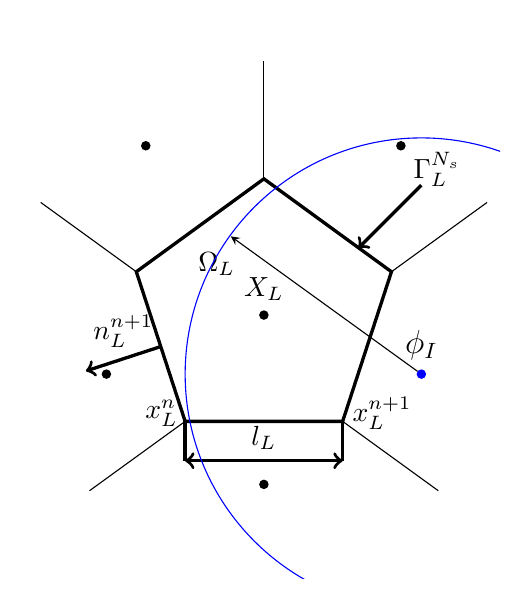
\begin{tikzpicture}[dot/.style={circle,inner sep=1pt,fill,label={#1},name=#1},
	extended line/.style={shorten >=-#1,shorten <=-#1},
	extended line/.default=1cm,
	one end extended/.style={shorten >=-#1},
	one end extended/.default=1cm,
	]
	\draw [extended line=1.5cm] (0,0) -- (2.62,1.90);
	\draw [extended line=1.5cm] (-0.62,1.90) -- (2,0);
	\draw (1,3.08) -- (1,4.58);
	%Front View
	\filldraw[fill=white,very thick](0,0) -- (2,0) -- (2.62,1.90) -- (1.00,3.08) -- (-0.62,1.90) -- (0,0);
	\draw [->,very thick] (3,3) -- (2.2,2.2);
	\node at (3.2,3.2) {$\Gamma_L^{N_s}$};
	%draw nodes
	%	\node at (0,0) circle(2pt) {A};
	\node[circle,draw=black, fill=black, inner sep=0pt,minimum size=3pt,label={$X_L$}] (a) at (1,1.35) {};
	\node[circle,draw=black, fill=black, inner sep=0pt,minimum size=3pt] (b) at (-1,0.6) {};
	\node[circle,draw=blue, fill=blue, inner sep=0pt,minimum size=3pt,label={\large {$\phi_I$}}] (c) at (3,0.6) {};
	\draw[->,>=stealth] (c) -- (0.58,2.35);
	\node[circle,draw=black, fill=black, inner sep=0pt,minimum size=3pt] (d) at (1,-0.8) {};
	\node[circle,draw=black, fill=black, inner sep=0pt,minimum size=3pt] (e) at (-0.5,3.5) {};
	\node[circle,draw=black, fill=black, inner sep=0pt,minimum size=3pt] (f) at (2.74,3.5) {};
	\node (1a) at (0.4,2) {$\Omega_L$};
	\draw [very thick] (0,0) -- (0,-0.5);
	\draw [very thick] (2,0) -- (2,-0.5);
	\draw [<->,very thick] (0,-0.5) -- node[above] {$l_L$} ++(2,0);
	\draw[->,very thick] (-0.31,0.95) -- node[above] {$n_L^{n+1}$} ++(-0.95,-0.31);
	\node (1a) at (-0.3,0.1) {$x_L^{n}$};
	\node (1a) at (2.5,0.1) {$x_L^{n+1}$};
	
	\begin{scope}
	\clip (-2,-2) rectangle (4,5);
	\draw[draw=blue](3,0.6) circle(3);
	\end{scope}
	\end{tikzpicture}%
	\vspace{0.25cm}
	\caption{Voronoi Diagram} \label{fig:M1}  
\end{figure}  




\chapter{Design}
\section{Domain}

\subsubsection*{Overview}
The domain package is intended to hold together the geometric details of the problem, i.e the nodes, the intergration cells and the degrees of freedom attached to the domain. From this other packages will reference this domain, such as the meshfree packaage, which builds the meshfree domain, and the integration package.
The domain is described by the structure 

\begin{tcolorbox}
	\begin{lstlisting}
	type Domain struct {	
		Name string // name the domain
		Nodes []node.Node // nodes within the domain
		num_nodes int // number of nodes
		voronoi *voronoi.Voronoi // Voronoi diagram
		dim int // dimension of domain
		boundaryNodes []int // index of nodes on boundary
		global_basis *[]*Dir //basis vectors e.g <1,0> <0,1> for 2D 
	}
	\end{lstlisting}
\end{tcolorbox}

At present there are two ways to build a domain, manually by adding nodes to a domain object, or more simply by providing a planar-straight line graph (PLSG) to the domain constructor, given by:
\begin{tcolorbox}
\begin{lstlisting}
domain := domain.DomainNew(fileName string, options string, dim int, global_coordinate coordinateSystem)
\end{lstlisting}
\end{tcolorbox}

Where $fileName$ is the name of the PLSG, $options$ provides a set of rules the mesh, and voronoi generator, see \url{https://www.cs.cmu.edu/~quake/triangle.html} for a description. The variable $dim$ ensures that correct number of degrees of freedom(DOFs) will be set. The coordinate system can be generated using the following function (for Cartesian coordinates),
\begin{lstlisting}
globalCS := coordinatesystem.CreateCartesian()
\end{lstlisting}
axisymmetric (cylindrical coordinates) are also supported. This function will construct the nodes, the degrees of freedom (assuming they are all free to start with) and the Voronoi diagram, which is used in the stabalised nodal integration scheme (SCNI).

\subsubsection*{Public functions}
In this section the public functions available to a domain object are described
\begin{lstlisting}
func (domain *Domain) GetDim() int 
\end{lstlisting}
Returns the dimensions of the Domain object $domain$
\begin{lstlisting}
func (domain *Domain) SetCoordinateSystem() 
\end{lstlisting}
Sets the coordinate system of the Domain object $domain$
\begin{lstlisting}
func (domain *Domain) AddNodes(nodes ...*node.Node) 
\end{lstlisting}
Appends the nodes to the domain and increments the number of nodes counter
\begin{lstlisting}
func (domain *Domain) GetNumNodes() int 
\end{lstlisting}
Returns the number of nodes in the domain
\begin{lstlisting}
func (domain *Domain) GetNodesIn(shape * geometry.Shape) *[]*Node
\end{lstlisting}
Returns the nodes inside the shape interface, e.g square, circle, cylinder.
\begin{lstlisting}
func (domain *Domain) TriGen(filename string, options string)
\end{lstlisting}
Triangulates the domain defined by the planar-straight line graph (PLSG). Uses the Triangle programme written in C.
\begin{lstlisting}
UpdateDomain
\end{lstlisting}
\begin{lstlisting}
CopyDomain
\end{lstlisting}
\begin{lstlisting}
CreatDofs
\end{lstlisting}
\begin{lstlisting}
func (domain *Domain) GenerateClippedVoronoi()
\end{lstlisting}
Generates a clipped voronoi diagram using JC\_VORONOI to construct the voronoi diagram, and the general polygon clipper (GPC) to clip the resulting diagram. Both libraries are written in C. 
\begin{lstlisting}
func GetVoronoi
\end{lstlisting}
Returns a pointer to the Voronoi diagram within the domain.

\begin{lstlisting}
PrintNodesToImg
\end{lstlisting}

\subsubsection*{Private functions}
None so far

\pagebreak
\section{Shape functions}
The shape function routines are contained within the $shapefunctions$ package. The fundamental data structure in this routine is the meshfree structure, which is a 'layer' of meshfree information implemented on-top of the physical domain

\begin{tcolorbox}
	\begin{lstlisting}
	type Meshfree struct {	
		domain *domain.Domain // reference to the underlying physical domain
		nodalSpacing []float64 // distance to the closest node for each node 
		gamma []float64 // support size multiplier for each node
		isConstantSpacing bool// whether base domain sizes are the same
		isVariousPoints bool // whether finding basis functions at multiple points
		basisFunctionRadii []float64 // radius(support) of each basis function
		dim int // does not need to be here
		tol float64// tolerance for maxent convergence
	}
	\end{lstlisting}
\end{tcolorbox}
\noindent To construct a meshfree structure the following constructing function can be used:
\begin{lstlisting}
func NewMeshfree(domain *domain.Domain, isConstantSpacing bool, isVariousPoints bool, dim int, gamma []float64, tol float64)
\end{lstlisting}
if the support size parameter ($gamma []float64$) is left empty it can be set using the following functions:
\begin{lstlisting}
func (meshfree *Meshfree) SetConstantGamma(gamma float64)
\end{lstlisting}
if a constant gamma (same support size parameter for each node)
or 
\begin{lstlisting}
func (meshfree * Meshfree) setGamma(gamma []float64)
\end{lstlisting}
if the support size parameter is different for each node. Note: the length of gamma should be equal to the number of nodes in the domain. 


\subsubsection*{Private functions:}
\section{Geometry}


\section{Example}

	
\chapter{Furture Plans}
\chapter{Area of Improvements}	
As the matrix library (gonum) is based off the blas libaries the performance for smaller domains is expected to be poor due to the overhead of calling the blas routines. Therefore it may be best to rediesng the shape function library.
\chapter{Acknowledgements}
The following packages have been used in this project
\end{document}